\documentclass[a4j,10pt, twocolumn]{jarticle}
\usepackage[dvipdfmx]{graphicx}
\usepackage{amssymb}
\usepackage{amsmath}
\usepackage{float}
%\usepackage{slashbox}
%---------------------------------------------------
% ページの設定
%---------------------------------------------------
\setlength{\textwidth}{170truemm}
\setlength{\textheight}{250truemm}
\setlength{\topmargin}{-14.5truemm}
\setlength{\oddsidemargin}{-5.5truemm}
\pagestyle{empty}
\setlength{\headheight}{0truemm}
\setlength{\parindent}{1zw}

\begin{document}
\twocolumn
[
\begin{center}
{\huge 奈良先端大において取り組みたい研究テーマについて}
\end{center}
\begin{flushright}
\begin{tabular}{rr}
{\Large \ }
&試験区分: 情報科学区分\\
&氏名: 桝田修慎\\
&希望研究室: 生体医用画像研究室\\
&現在の専門: 深層学習\\
{\Large \ } 
\end{tabular}
\end{flushright}
\vspace{2truemm}
]
\section{これまでの修学内容}
学部では1年次に線形代数学・解析学など,専門的な学習を始めるために必要な基礎を学び,2年次からは人工知能基礎・応用,データベース,自然言語処理など専門的な講義が開講され,積極的に受講した.
そしてこの時期から,将来取り組みたい分野を見つけるきっかけ作りとして,資格取得に向けて学習をはじめ,基本情報技術者試験・応用情報技術者試験を取得した.
4年次の研究室配属では第一志望であった,脳型情報処理や人工知能を専門としている研究室に配属され,Vision Transformerを用いた画像解析の研究をしている.

\section{取り組みたい研究テーマ}
私が,奈良先端大において取り組みたい研究テーマは「Self Attentionを用いた生体医用画像のマルチモーダルセグメンテーション」である.本稿では,この研究テーマの研究背景,研究課題,提案手法,期待される結果について述べる.
\section{研究の背景}
近年,ディープラーニング技術は実務レベルの利用が急速に拡大しており,医療分野にも多く応用されている.
中でも「診断支援」の領域では,ディープラーニングの持つ特徴抽出能力を用いることで,生体医用画像から病変のある箇所を抽出する技術が注目されており,コンピュータ診断支援 (Computer-Aided Diagnosis : CAD)と呼ばれている. 
この技術は「医師への負担を緩和させ,病変の見落としリスクを低減させる」ことが目的であるが,病変箇所と解剖学的構造物が重なった場合や,病変の規模が小さい場合は抽出することが困難である.
そのため,誤診断や医師による二重チェックなどが発生し,根本的な解決には至っていない.
%また,CADに使われるモデルの多くはU-netであり,ConvolutionとDownsampling,経験豊富な医師に匹敵する精度で異常箇所を発見することが可能になってきている.しかし一方で,モデルの学習に膨大な時間がかかることが懸念されている.

病変部位を抽出する手法としてセグメンテーションが用いられることが多く,最近ではU-netを利用した研究が頻繁に行われている\cite{近藤堅司2018u}.
U-netでは,畳み込み層を重ねることで失われていく画像構成要素の位置情報を,SkipConectionによって保持することができるが,セグメンテーションしたい対象が重なっている場合や複数ある場合に効果を発揮しづらい.
その問題を解決するために,インスタンスごとにセグメンテーションを行うモデルが開発され,Mask R-CNNと呼ばれている\cite{he2017mask}.
魚住らの研究によるとMask R-CNNのモデルは小児胸部X線画像における肺領域の自動抽出においてU-netより低い抽出精度を示していたものの,肺炎による炎症の広がりがある症例において正確に肺野を抽出していた\cite{魚住春日2020mask}.
このことから,Mask R-CNNの抽出精度を向上させることができれば,過剰抽出や欠損が無いロバスト性の高いモデルができると予想される.

\section{研究課題}
上述の通り画像による診断支援を実務で利用するには,精度の向上を目指すべきである.
そのためには先に記した通り,解剖学的構造同士の重なりや,病変部位との重なりによる誤診断をどのように解決するかを考える必要がある.

\section{提案手法}
私は二つの視点から医用画像を解析する手法 (図1) を提案する.一つ目は自然言語処理のSelf Attention\cite{vaswani2017attention}.二つ目は画像処理のMask R-CNN.
これらを組み合わせ,文章と画像双方からアプローチを行うことにより,正確に病変セグメンテーションができると私は考える.

\begin{figure}[ht]%default85mm
    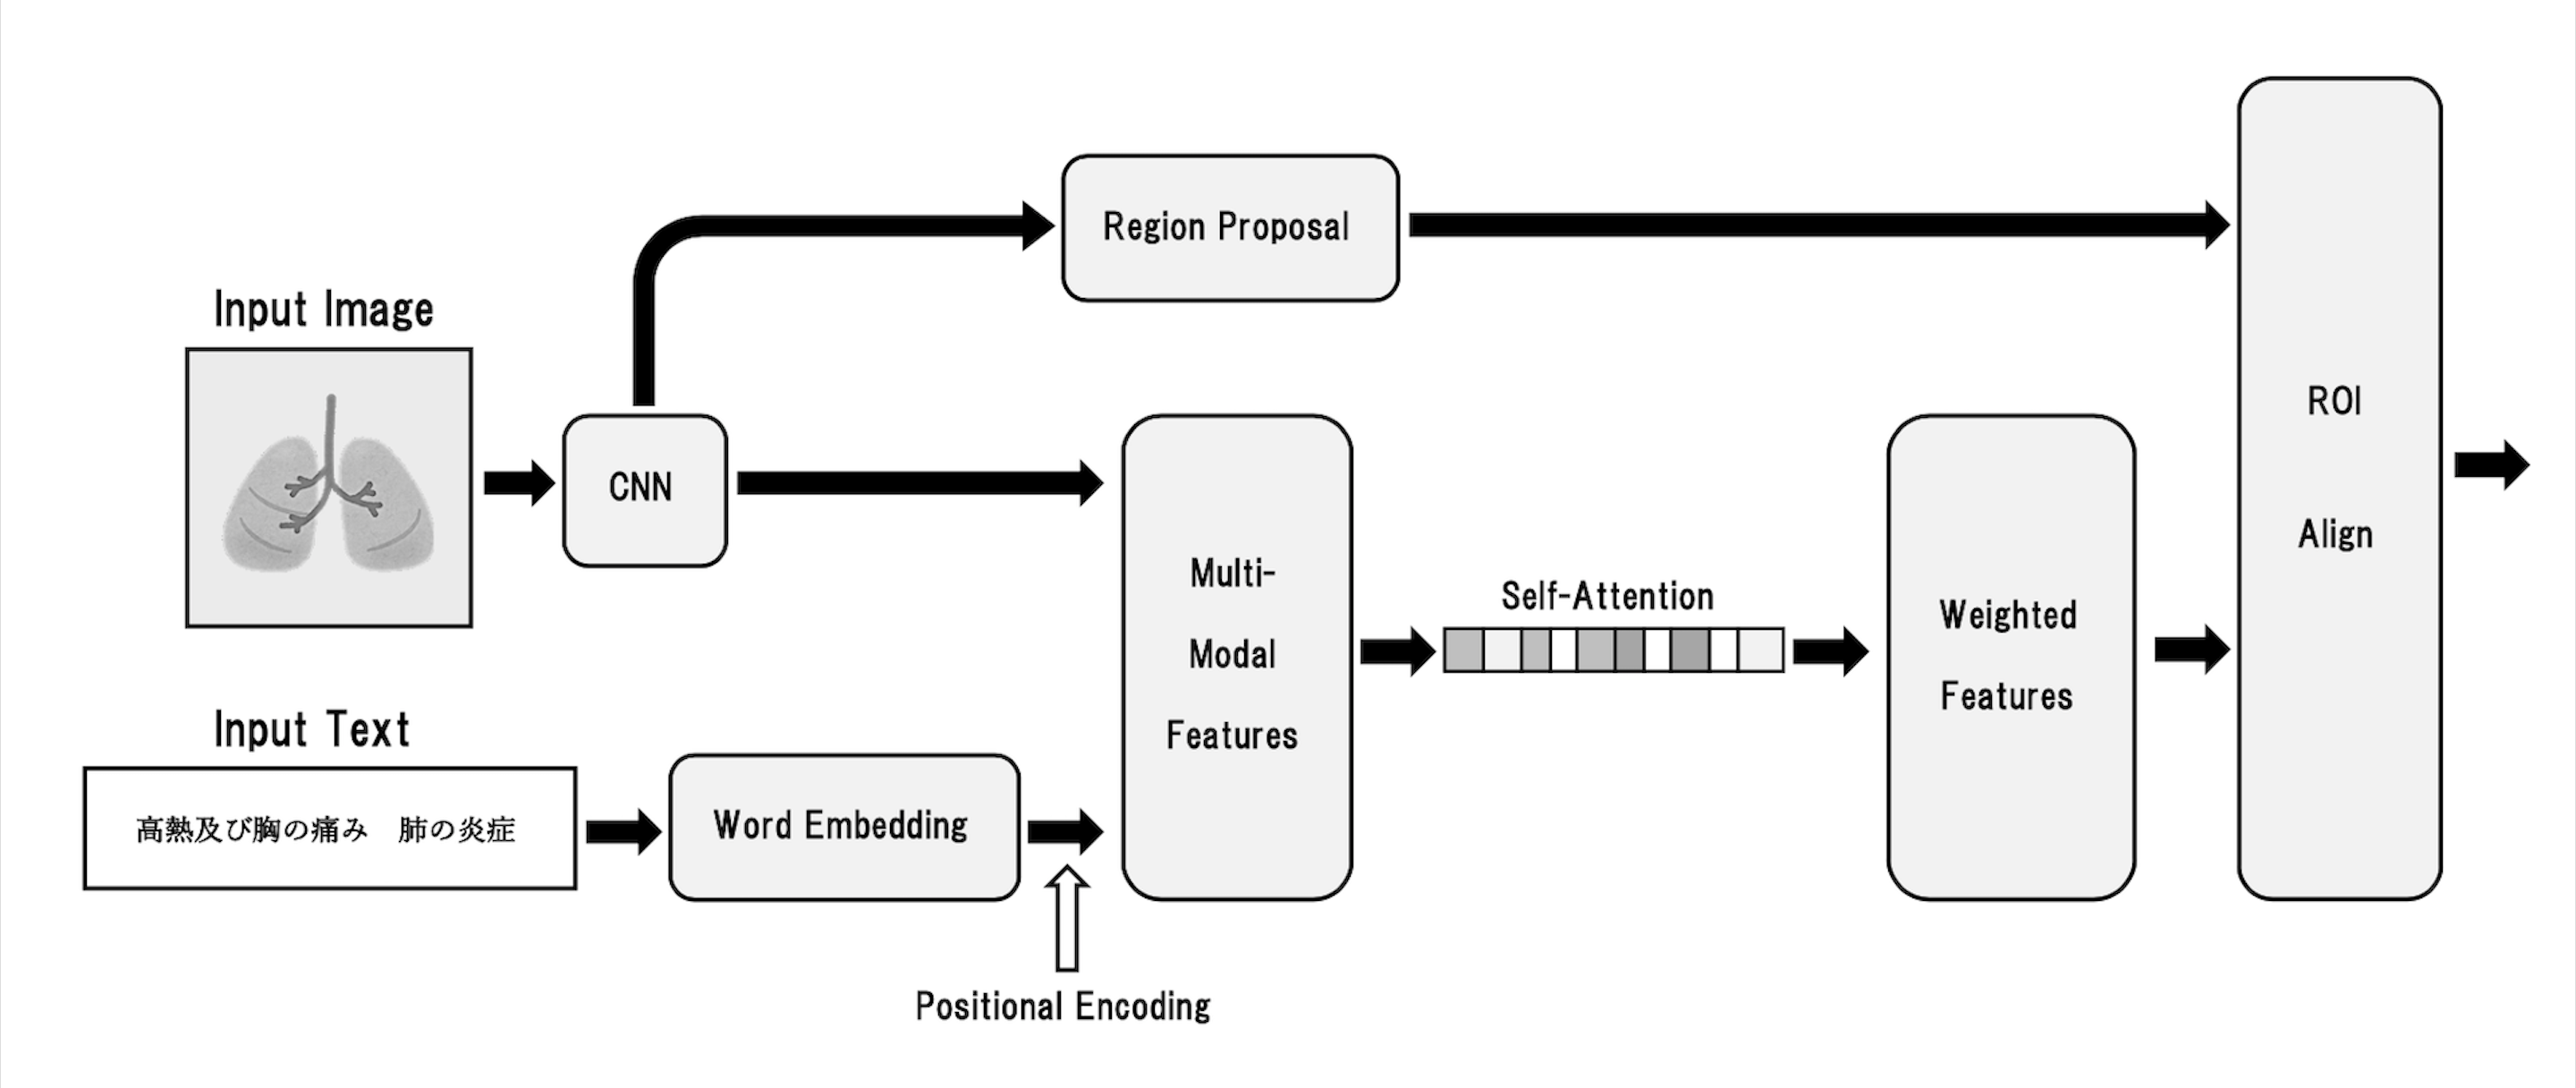
\includegraphics[width=80mm]{/Users/markun/git/NAIST_essay/mask4.png}
    \caption{マルチモーダルなセグメンテーションの流れ}
\end{figure}

\twocolumn
[
%\begin{center}
%{\huge 奈良先端大において取り組みたい研究テーマについて}
%\end{center}
\begin{flushright}
\begin{tabular}{rr}
{\Large \ }
&試験区分: 情報科学区分\\
&氏名: 桝田修慎\\
&希望研究室: 生体医用画像研究室\\
&現在の専門: 深層学習\\
{\Large \ } 
\end{tabular}
\end{flushright}
\vspace{2truemm}
]

図1はMask R-CNNのアーキテクチャの一部を抜粋し改変したものである.

ここでは,画像と文章の入力から,すでに提案されているMask R-CNNのアーキテクチャに接続するまでの処理を説明する.
初めに,患者の症状や想定される疾患を文章として与えてWord Embedding\cite{堅山耀太郎2017word}により固有のベクトルに落とし込み, Positional Encodingにより位置情報を付加する.これにより得られたベクトルを特徴量として,CNNで得られた特徴量と組み合わせ,Multi modal featuresとして扱う.
次はMulti modal featuresを元にSelf Attentionを求める.
図1の例では,入力文章として「高熱及び胸の痛み 肺の炎症」を与え,それぞれのSelf Attentionを求めている.この場合Attentionは「肺」,「炎症」などで大きくなり,「及び」,「の」で小さくなると考えられる.
以上により得られたAttentionを元の特徴量に掛け合わせてWeighted featuresを算出.
また,RPN(Region Proposal Network)\cite{ren2015faster}によって得られたRegion ProposalをWeighted featuresと共にROI Align(Region Of Interest Align)に入力し特徴量を得る,という流れだ.
その後,通常のMask R-CNNと同様に,Mask branchとFully connected layerを経てセグメンテーションされた出力が得られる.
\section{期待される結果}
私が提案するSelf Attentionを用いた手法は,CNN単体で特徴量を抽出した場合に比べ,病気に対する情報を多く保持していると予想されるので,過剰抽出や欠損の少ない結果が安定して得られると考える.
また,Self Attentionを求めていることから,画像・文章のどこに注目しているかを可視化できるので,患者に対する病症の説明も比較的容易になると予想される.
%\section{まとめ}

\section{最後に}
本稿では,私が奈良先端大で取り組みたい研究テーマである「Self Attentionを用いた生体医用画像のマルチモーダルセグメンテーション」の研究概要について述べてきた.
私が奈良先端大を志望するのは,医用画像工学を学べる数少ない大学院の一つであり,学部を持たずに様々なバックグラウンドをもった人間を受け入れていて,そのサポートも充実しているからだ.
また,全ての講義が英語で行われており,早期からグローバルに活躍するための力を養うことができ,同時に高度な技術力を身につけられる環境が備わっているのも志望動機のひとつである.

\bibliographystyle{jplain}
\bibliography{/Users/markun/git/NAIST_essay/reference.bib}

\end{document}